\chapter{Povezovalna pravila}

Danes vse prodajalne, tako spletne kot te, kamor se moramo sprehoditi ali pa zapeljati z nekim prevoznim sredstvom, beležijo podatke o nakupih. Te, ki tega ne počno, so že propadle ali pa so žal na poti propada. Recimo, prodajalna prehrambenih izdelkov. Oglejmo si en zelo majhen vzorec nakupov  (tabela~\ref{t:transakcije}), kjer vsaka vrstica prikazuje, kaj je bilo v nakupovalni košarici. V tem poglavju bomo zadeve zelo poenostavili: kupci bodo ostali anonimni, čas nakupa nas ne bo zanimal, prav tako ne bomo beležili števila nakupljenih stvari. Zanimali nas bodo samo tipi nakupljenih stvari v nakupovalnih košaricah (na primer, mleko, ne pa tri litri mleka, in ne pol štruce kruha).

\begin{table}
\caption{Podatki o nakupovalnih košaricah.}
\label{t:transakcije}
\begin{center}
\small
\begin{tabular}{lll}
\toprule
nakup & stvari v košarici & poenostavljen zapis \\
\midrule
$t_1$ & mleko, kruh & MK \\
$t_2$ & mleko, sir, zelenjava & MSZ \\
$t_3$ & kruh, sir, zelenjava & KSZ \\
$t_4$ & mleko, kruh, sir, zelenjava & MKSZ \\
$t_5$ & mleko, kruh, sir & MKS \\
$t_6$ & kruh, sir & KS \\
$t_7$ & sir & S \\
$t_8$ & kruh, zelenjava, sir & KZS \\
$t_9$ & sir, zelenjava & SZ \\
$t_{10}$ & kruh, sir, zelenjava & KSZ \\
\bottomrule
\end{tabular}
\end{center}
\end{table}

Nakupovalne košarice smo označili s $t_i$ za $i$-to nakupovalno košarico. Bolj strokovno vsaki vrstici v tabeli~\ref{t:transakcije} pravimo tudi {\em transakcija}. Naj bo množica transakcij, katero bi želeli preučiti, ${\mathcal T}=\{t_1,t_2,\ldots t_N\}$. Množico stvari, ki lahko nastopajo v teh transakcijah, označimo z ${\mathcal I}=\{i_1,i_2,\ldots i_M\}$.

\section{Nabori in podnabori}

Terkam stvari, kot so na primer \{kruh, sir\} ali pa \{mleko, sir, zelenjava\} pravimo {\em nabor}. Za par naborov $X$ in $Y$ pravimo, da je $X$ podnabor nabora $Y$, če je vsaka stvar iz nabora $X$ vsebovana v naboru $Y$. V tem primeru zapišemo, da velja $X\subseteq Y$. Nabor \{kruh, sir\} je na primer podnabor nabora \{kruh, mleko, sir\}. Števnost stvari v naboru $X$ označimo $|X|$. V naboru $X=\{{\rm kruh}, {\rm mleko}, {\rm sir}\}$ so tri stvari, $|X|=3$. Nabor $X$ s števnostjo $|X|$ ima $2^{|X|}$ možnih podnaborov, med katerimi je tudi prazen podnabor $\emptyset$.

\section{Podpora in pogosti nabori}

S $\sigma(X)$ označimo število transakcij, ki vsebuje podnabor $X$. Podnabor $X=\{{\rm mleko}, {\rm kruh}\}$ je vsebovan v transakcijah $t_1$, $t_4$ in $t_5$. Število podprtih transakcij za nabor $X$ je zato enako tri, oziroma $\sigma(X)=3$. Število $\sigma(X)$ formalno določimo s sledečim zapisom:
%
\begin{equation}
  \sigma(X)=|\{t_i|X\subseteq t_i, t_i\in {\mathcal T}\}|
\end{equation}

Iz števila podprtih transakcij za nabor $X$ lahko izračunamo delež podprtih transakcij, torej delež transakcij, ki vsebujejo nabor $X$:
%
\begin{equation}
  s(X)={\sigma(X)\over |{\mathcal T}|}={\sigma(X)\over N}
\end{equation}

Zanima nas, kateri nabori so taki da za njih velja
\begin{equation}
  s(X)\geq{\rm minsupp}
\end{equation}
kjer je ${\rm minsupp}$ minimalna podpora oziroma parameter, ki ga določi uporabnik. Nabore, kjer velja zgornji izraz, imenujemo {\em pogosti nabori}.

\section{Algoritem Apriori}

Za iskanje vseh pogostih naborov v množici transakcij bomo razvili algoritem Apriori, ki sta ga sicer predlagala Agrawal in Srikant leta 1994. A preden zapišemo algoritem, razmislimo o nekaj lastnostih prostora vseh možnih naborov. Ti so za naš primer grafično prikazani v mreži naborov (slika~\ref{f:mreza-naborov}), kjer so nabori določenega nivoja povezani z nabori prejšnjega nivoja, če so slednji njihovi podnabori. Tako je vozlišče MKZ povezano z vozlišči MK, MZ in KZ, a ne z vozliščem MS, saj MS ni podnabor MKZ.

\begin{figure}[htbp]
\centering{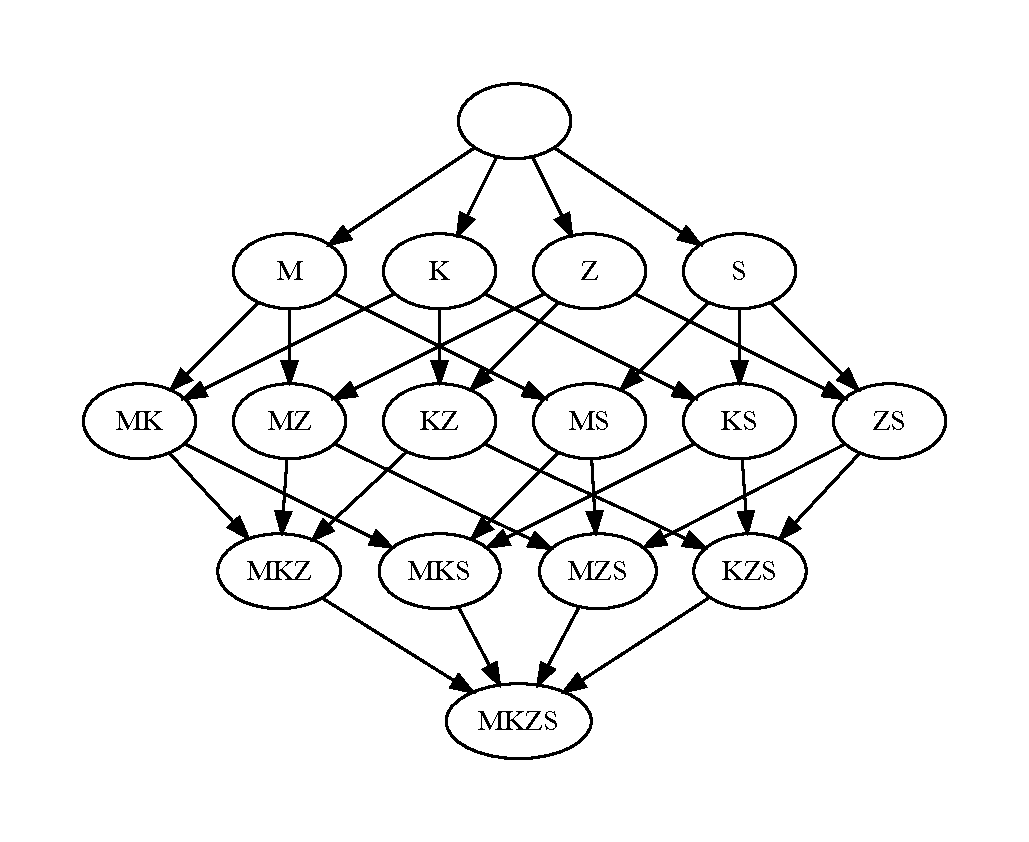
\includegraphics[width=9cm]{slike/mreza-naborov.pdf}}
\caption{Mreža vseh možnih naborov za množico stvari mleko (M), kruh (K), zelenjava (Z) in sir (S). V korenu grafa je prazen nabor.}
\label{f:mreza-naborov}
\end{figure}

Recimo, da iščemo pogoste nabore s podporo vsaj 0.6 (${\rm minsupp}=0.6$). Najprej za vsak nabor v mreži naborov določimo število transakcij, v katerih je ta nabor prisoten. Za naš primer tako označeno mrežo prikazuje slika~\ref{f:mreza-pogostih-naborov}. Pogosti nabori morajo biti vsebovani vsaj v šestih transakcijah. Iz mreže je razvidno, da to velja za šest naborov, med katerimi je eden prazen.

Iz mreže naborov lahko razberemo nekaj zanimivih zakonitosti. Recimo, nabor M je nepogost. Zaradi tega so nepogosti prav vsi nabori z mlekom, torej vsi nabori, katerih podnabor je M. To je razumljivo, saj vsi ti nabori zahtevajo, da je njhov podnabor tudi M, ta pa je vsebovan v pramajhnem številu transakcij, da bi bili nabori, ki ga vsebujejo, pogosti.

Prav tako razberemo, da podpora nabora ne more presegati podpore kateregakoli njegovega podnabora. Primer: KZS je vsebovan v štirih transakcijah, in to število ne sme presegati števila transakcij, v katerih so vsebovani vsi njegovi možni podnabori, torej tudi ti iz prejšnjega nivoja (KZ, KS, ZS).

\begin{figure}[htbp]
\centering{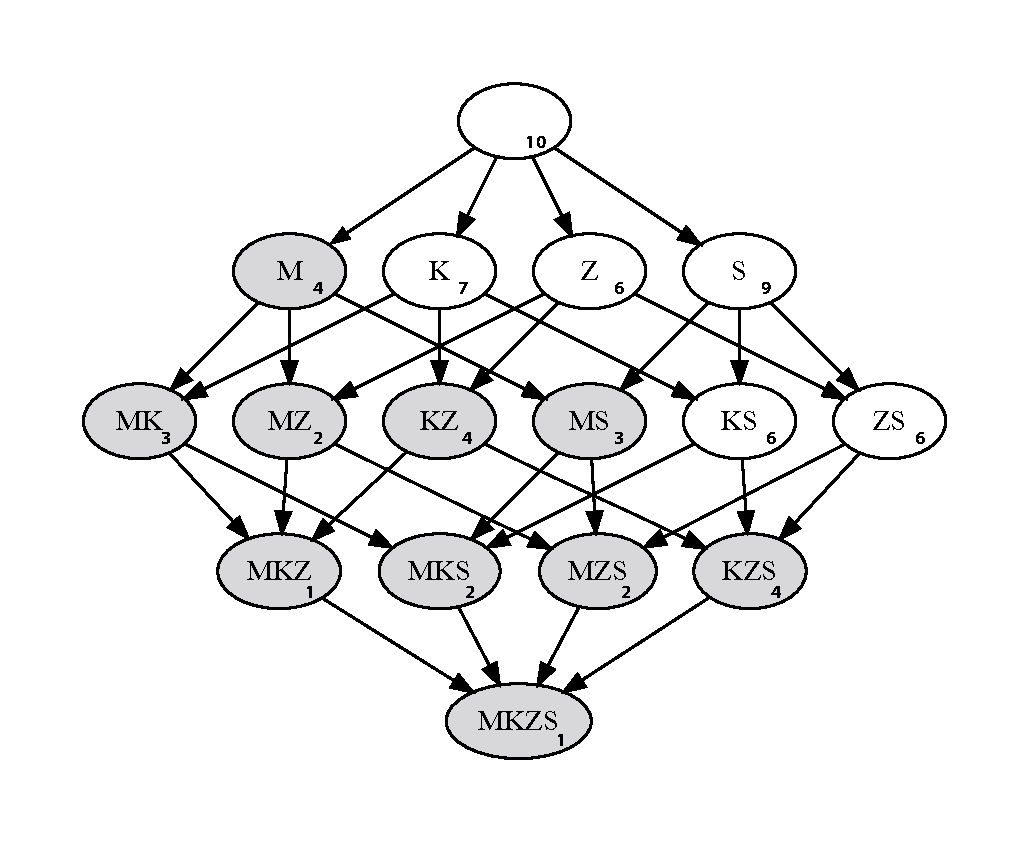
\includegraphics[width=9cm]{slike/mreza-pogostih-naborov.pdf}}
\caption{Mreža pogostih naborov (naborov v praznih vozliščih) za ${\rm minsupp}=0.6$ oziroma za vse nabore, katerih število podpornih transakcij je vsaj 6 ($6=0.6\times 10$). Vozlišča, ki predstavljajo nepogoste nabore, so osenčena.}
\label{f:mreza-pogostih-naborov}
\end{figure}

Zgornja zapažanja zapišimo v obliki teoremov.

\begin{teorem}
  Če je nabor pogost, so pogoste tudi vse njegove podmnožice:
  $$s(X)\geq{\rm minsupp}\implies s(Y)\geq{\rm minsupp}, Y\subseteq X$$
\end{teorem}

\begin{teorem}
  Če je nabor nepogost, so nepogosti tudi vsi nabori, ki ga vsebujejo:
  $$s(X)<{\rm minsupp}\implies s(Y)<{\rm minsupp}, X\subseteq Y$$
\end{teorem}

\begin{teorem}
  Podpora nabora nikoli ne presega podpore njegove podmnožnice (antimonotonost, ${\mathcal L}=2^I$ je močnostna množica, torej množica vseh možnih naborov):
  $$ \forall X,Y\in {\mathcal L}: X\subseteq Y\implies s(Y)\leq s(X) $$
\end{teorem}

Iz zgornjega intuitivno sledi algoritem Apriori. Ker nas prazna množica ne zanima, pričnemo lahko s pogostimi nabori prvega nivoja, torej nabori, ki vsebujejo natanko eno stvar (te imenujemo tudi {\em pogosti 1-nabori}). Od tu dalje s kombinacijo pogostih naborov generiramo {\em pogoste $k$-nabore}, kjer $k$ iterativno povečujemo. Ustavimo se, ko na $k$-tem nivoju ni več pogostih naborov, saj bi to pomenilo, da teh tudi ni v vseh višjih nivojih.

\begin{tabbing}
xxx\=xxx\=xxx\=xxx \kill\\
{\bf Vhod}: množica transakcij in minimalna podpora minsupp \\
{\bf Izhod}: množica pogostih naborov \\
\\
$k=1$ \\
$F_k=\{i|i\in I\land\sigma(i)\geq N\times{\rm minsupp}\}$ \\
{\bf ponavljaj} \\
\> $k\leftarrow k+1$ \\
\> $C_k={\rm kandidati}(F_{k-1})$ \\
\> izračunaj podporo naborov v $C_k$ \\
\> $F_k=\{c | c\in C_k\land\sigma(c)\geq N\times{\rm minsupp}\}$ \\
{\bf dokler} $F_k=\emptyset$ \\
{\bf vrni} $\cup_k F_k$ \\
\end{tabbing}

Algoritem Apriori uporablja funkcijo kandidati, ki na podlagi že odkritih pogostih naborov tvori pogoste $k$-nabore. S podrobnostmi implementacije te funkcije se ne bomo ukvarjali, omenimo pa samo, da so za hitrost celotnega algoritma precej pomembne. Namreč, izogniti se moramo tvorjenju enakih kandidatov. Recimo, nabor KS lahko tvorimo iz pogostega nabora K in stvari S, ali iz pogostega nabora S in stvari K. Tu omenimo samo nekaj možnosti, ki jih lahko pri tvorjenju kandidatov lahko uporabimo:
\begin{itemize}
\item Kandidate za $F_k$ tvorimo iz kombinacije pogostih naborov $F_{k-1}\times F_1$. Problem podvojenih kandidatov rešimo z leksikografsko ureditvijo naborov (na primer MKZ je z MZS, saj je K leksikografsko pred Z).
\item Kandidate za $F_k$ tvorimo iz kombinacije pogostih naborov $F_{k-1}\times F_1$, kjer nabora združimo le, če sta različna samo v zadnjem elementu. Tudi tu problem podvojenih kandidatov rešujemo z leksikografsko ureditvijo naborov.
\end{itemize}

\section{Povezovalna pravila}

Pravila tipa
$$ X\rightarrow Y $$
kjer sta X in Y nabora stvari, imenujemo {\em povezovalna pravilna}. Zahtevamo, da je presečna množica obeh naborov prazna, torej $X\cap Y=\emptyset$. Primer takega pravila je recimo
$$ {\rm kruh}\to {\rm mleko}, {\rm sir}$$
pravilo pa pravi, da če bo v košarici kruh, pričakujemo, da bosta tam tudi mleko in sir. Še en primer povezovalnega pravila je
$$ {\rm mleko}, {\rm sir}\to {\rm zelenjava} $$
ki pravi, da če bosta v košarici mleko in sir, pričakujemo, da bo tam tudi zelenjava.

Pravila so lahko seveda bolj ali manj v soglasju z učno množico transakcij. Povezovalna pravila ocenjujemo z merami, med katerima sta najbolj znani podpora in zaupanje. {\em Podporo} že poznamo, poroča pa o delež transakcij, kjer najdemo vse stvari iz povezovalnega pravila:
\begin{equation}
  s(X\to Y)={\sigma(X\cup Y)\over N}
\end{equation}
Podpora torej meri pogostost pravila v množici transakcij.

Drugačna mera je {\em zaupanje}, ki meri, kakšen je delež transakcij, ki vsebujejo desno stran pravila $Y$ med transakcijami, ki vsebujejo levo stran pravila $X$:
\begin{equation}
  c(X\to Y)={\sigma(X\cup Y)\over\sigma(X)}
\end{equation}

Za pravilo ${\rm M}\to {\rm SK}$ bo tako podpora enaka $0.2$, zaupanje pa enako $0.5$ (štiri transakcije vsebujejo mleko, od tega dve poleg mleka še sir in kruh). Podpora pravila ${\rm Z}\to{\rm S}$ bo $0.6$, zaupanje pa $1.0$.

Algoritmu za iskanje podpornih pravil predpišemo ${\rm minsupp}$ in ${\rm minconf}$, torej minimalno podporo in minimalno zaupanje. V praksi pa pravila iščemo tako, da najprej poiščemo pogoste nabore, potem pa iz teh izluščimo pravila, katerih zaupanje je dovolj visoko. Pogosti nabori bodo namreč imeli enako podporo kot pravila, ki vsebujejo vse stvari iz pogostega nabora. Iz nabora ${\rm KZS}$ lahko tako tvorimo $2^3-2=6$ netrivialnih pravil, kjer je leva oziroma desna stran pravila neprazna:

\begin{center}
  KZ$\to$S, KS$\to$Z, ZS$\to$K, \\
  S$\to$KZ, Z$\to$KS, K$\to$ZS
\end{center}

Za dani nabor stvari lahko tvorimo vsa možna povezovalna pravila na podoben način, kot smo tvorili vse možne podnabore. Z eno samo razliko. Tokrat podnabore v mreži uporabimo za desno stran povezovalnega pravila, na levo stran pa damo vse, kar je v naboru, ki ga cepimo v pravilo, še ostalo. Tako nam za nabor ${\rm KZS}$ mreža na sliki~\ref{f:pravila-kzs} podaja vse možne cepitve oziroma vsa možna pravila.

\begin{figure}[htbp]
\centering{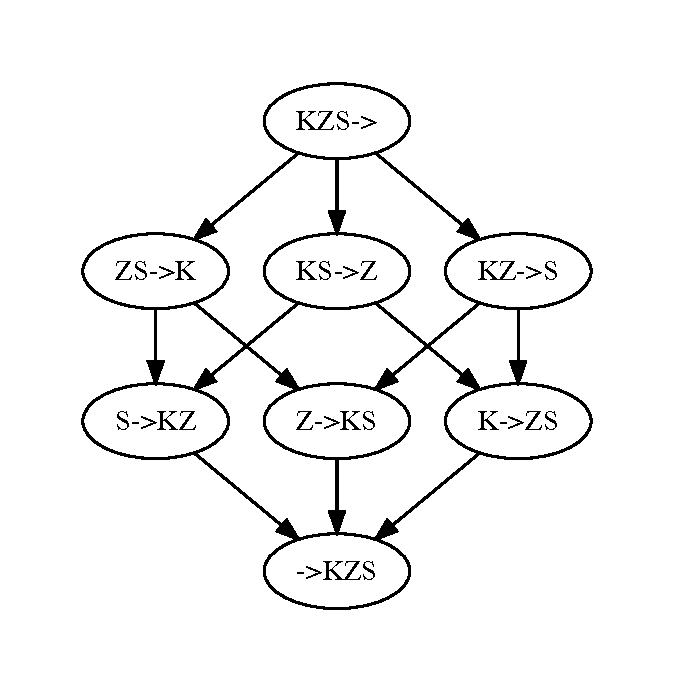
\includegraphics[width=9cm]{slike/pravila-kzs.pdf}}
\caption{Mreža vseh možnih povezovalnih pravil, ki jih lahko tvorimo iz nabora KZS. Pravili v korenu (prazen nabor na levi strani) in na zadnjem nivoju mreže nista legalni, sta pa vseeno prikazani.}
\label{f:pravila-kzs}
\end{figure}

Ostane nam le, da tudi tu poiščemo finto oziroma pristop, kjer je mrežo povezovalnih pravil graditi iz začetnega vozlišča tako, da kandidate klestimo glede na zahtevano zaupanje. V ta namen si oglejmo dve pravili, ki ju tvorimo iz nabora Z: ${\rm X}\to {\rm Z}-{\rm X}$ in ${\rm X'}\to {\rm Z}-{\rm X}'$. Vsakič smo torej desno stran pravila dobili tako, da smo od nabora ${\rm Z}$ odstranili stvari na levi strani pravila, ki so enkrat bile X in drugič ${\rm X}'$.

\begin{teorem}
  Naj bosta ${\rm X}$ in ${\rm X}'$, kjer je ${\rm X}'$ podnabor {\rm X}. Velja:
  $$c({\rm X}\to {\rm Z}-{\rm X})<{\rm minconf}\implies c({\rm X}'\to {\rm Z}-{\rm X}')<{\rm minconf} $$
\end{teorem}
Ta teorem moramo dokazati. Spomnimo se, da velja:
$$ {\rm X}'\subset {\rm X}\implies\sigma({\rm X}')\geq\sigma({\rm X}) $$
Neenačbo na desni strani pomnožimo z $\sigma(Z)$ in delimo z $\sigma({\rm X}')$ ter $\sigma({\rm X})$. Dobimo enačbi za zaupanje obeh pravil, in dokaz zgornjega teorema:
$${\sigma({\rm Z})\over\sigma({\rm X}')} < {\sigma({\rm Z})\over\sigma({\rm X})}$$

Z drugimi besedami: če ${\rm X}\to Z-X$ ne presega minimalnega zaupanja, tudi ${\rm X'}\to {\rm Z}-{\rm X}'$ ne bo, kjer je ${\rm X}'$ podnabor ${\rm X}$. V naši mreži povezovalnih pravil s slike~\ref{f:pravila-kzs} vidimo, da so pravila s podnabori levih strani postavljena v spodnjih nivojih pravil nivoja nad njimi. Če pravilo ZS$\to$K ne bo ustrezalo pogoju zaupanja, tudi pravili S$\to$KZ in Z$\to$KS, ki iz njega sledita, ne bodo.

Ravno smo torej ``izumili'' pristop gradnje povezovalnih pravil. Gradimo jih iz pogostega nabora. Uporabimo mrežo pravil, kjer pričnemo s prazno desno stranjo pravila in tej, na vsakem nivoju, dodamo po eno stvar ter na ta način tvorimo vse možne kombinacije. Pravila na nivoju $k$ gradimo s kombinacijo pravil nivoja $k-1$. Kot pri algoritmu Apriori tudi tu na vsakem nivoju hranimo samo pravila, ki ustrezajo kriteriju zaupanja.

Za velike množice transakcij gradnja povezovalnih pravil lahko privede do nepreglednih množic pravil. To se seveda zgodi pri premalo ostrih pogojih, torej pri premalo visokih minsupp in minconf. Taka pravila je ročno nemogoče pregledati. Pomagamo si tako, da skušamo najprej zmanjšati množico pogostih naborov z dvigovanjem minsupp, potem pa iz nje tvorimo pravila tako, da najprej skušamo postavljati bolj ostre pogoje za zaupanje. 
